\subsection{Unscented Kalman Filter on Manifolds}
\subsubsection{Concept and Motivation}
Up to this point, all Kalman Filter variants, including the EKF and ESKF, approximate nonlinear systems locally through 1st order linearization. Although effective for mildly nonlinear dynamics, these methods rely on Jacobians, which introduce errors when the system exhibits strong nonlinearity or discontinuous dynamics. An alternative approach to local linearization is sampling based nonlinear approximation. A well known technique of this class is the \textit{``Unscented Transform (UT)''}, which represents a Gaussian distribution using a small, deterministically chosen set of sample points (called sigma points) and then propagates them through the nonlinear function to capture the transformed mean and covariance up to the third order for Gaussian inputs \cite{ukf}.
\begin{figure}[H]
    \centering
    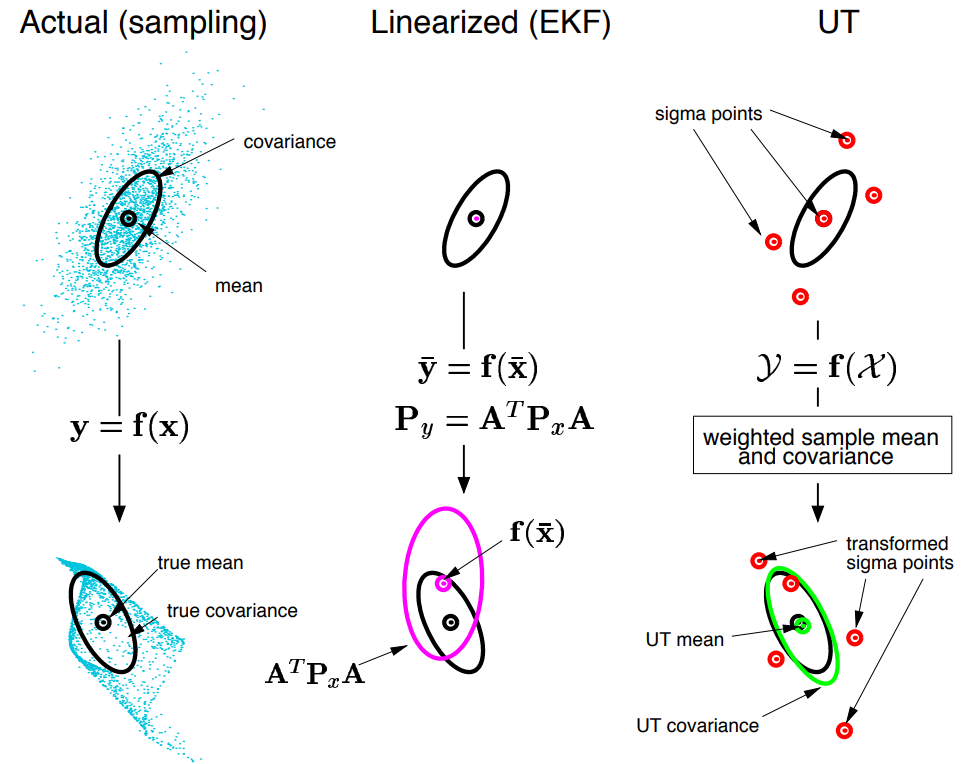
\includegraphics[width=0.7\linewidth]{Pictures/State_Estimation/Unscented_Kalman_Filter_on_Manifolds/Unscented_Transform.png}
    \caption{Comparison of different methods for nonlinear mean and covariance propagation. The figure contrasts (a) direct sampling of the true nonlinear distribution, (b) linearization using the Extended Kalman Filter (EKF), and (c) the Unscented Transform (UT), which captures the mean and covariance more accurately without linearization. Image taken from Unscented Kalman Filter paper.\textsuperscript{\cite{ukf}}}
    \label{fig:state-estimation-uncented-transform}
\end{figure}



\subsubsection{Unscented Kalman Filter}
The Unscented Transform is defined by generating a set of $2L + 1$ sigma points from the prior mean $\mathbf{x}$ and covariance $P$, where $L$ denotes the dimensionality of the state vector. Each sigma point represents a deterministic sample capturing the local mean and covariance structure of the state distribution, ensuring accurate nonlinear propagation up to the second order for any nonlinearity.
$$
\begin{aligned}
    \chi_0 &= \mathbf{x} \\
    \chi_i &= \mathbf{x} + (\sqrt{(L + \lambda)P})_i              && i = 1, \ldots, L \\
    \chi_i &= \mathbf{x} - (\sqrt{(L + \lambda)P})_{i - L}        && i = L+1, \ldots, 2L
\end{aligned}
$$
$$
    \lambda = \alpha^2 (L + \kappa) - L
$$
where $\lambda$ is a scaling parameter controlling the spread of the sigma points. Each sigma point is assigned associated weights $W_i^m$ and $W_i^c$ for mean and covariance reconstruction. These weights ensure that both the central and surrounding sigma points contribute correctly to the nonlinear mean and covariance propagation according to their statistical significance. The weights are defined as
$$
\begin{aligned}
    W_0^m &= \frac{\lambda}{L + \lambda} \\
    W_0^c &= \frac{\lambda}{L + \lambda} + (1 - \alpha^2 + \beta) \\
    W_i^m &= W_i^c = \frac{1}{2(L + \lambda)}                           && i = 1, \ldots, 2L
\end{aligned}
$$
The parameters $\alpha$, $\beta$, and $\kappa$ govern the spread, scaling, and higher order accuracy of the sigma point distribution. According to the original Unscented Kalman Filter formulation by Julier and Uhlmann \cite{ukf}, these parameters should be tuned to balance numerical stability and approximation accuracy. The parameter $\alpha$ determines the overall spread of the sigma points around the mean, it is typically chosen as a small positive value ($10^{-3} \leq \alpha \leq 1$), with smaller values resulting in sigma points closer to the mean and larger values increasing the nonlinear coverage at the cost of potential numerical instability. The parameter $\kappa$ acts as a secondary scaling term that adjusts the effective spread of the sigma points; it is often set to $0$ for simplicity or $3 - L$ to guarantee positive semi definiteness of the covariance. The parameter $\beta$ encodes prior knowledge of the underlying distribution, for Gaussian distributions, $\beta = 2$ is recommended, as it ensures optimal 2nd order accuracy in the covariance reconstruction. 
\\ \\  
Together, these parameters define how the sigma points are positioned and weighted to best approximate the true nonlinear mean and covariance transformation while maintaining numerical stability across a wide range of system non-linearities. 
\\ \\  
Using these sigma points and weights, the propagated mean and covariance are computed as
$$
\begin{aligned}
    \hat{\mathbf{x}}^- &= \sum_{i=0}^{2L} W_i^m f_d(\chi_i, \mathbf{u}) \\
    P^- &= \sum_{i=0}^{2L} W_i^c [f_d(\chi_i, \mathbf{u}) - \hat{\mathbf{x}}][f_d(\chi_i, \mathbf{u}) - \hat{\mathbf{x}}]^\top
\end{aligned}
$$
This process effectively replaces linearization and analytical Jacobian computation with a deterministic sampling of the nonlinear function. A similar procedure is applied during the measurement update step, where the sigma points are propagated through the nonlinear measurement model $h(\mathbf{x})$ to compute the predicted observation mean and covariance.
\\ \\
During the measurement update step, each predicted sigma point $\chi_i^-$ is passed through the nonlinear measurement model $h(\mathbf{x})$ (for example, the GNSS measurement model in Equation \ref{eq:aiding-measurement-model}) to get predicted measurement samples:
$$
    \mathcal{Z}_i = h(\chi_i^-)
$$
The predicted measurement sample mean is computed as
$$
    \hat{\mathbf{z}} = \sum_{i=0}^{2L} W_i^m \, \mathcal{Z}_i
$$
The corresponding innovation covariance and cross covariance are then obtained as
$$
    S = \sum_{i=0}^{2L} W_i^c \, (\mathcal{Z}_i - \hat{\mathbf{z}})(\mathcal{Z}_i - \hat{\mathbf{z}})^\top + R
$$
$$
    P_{xz} = \sum_{i=0}^{2L} W_i^c \, (\chi_i^- - \hat{\mathbf{x}}^-)(\mathcal{Z}_i - \hat{\mathbf{z}})^\top,
$$
where $R$ is the measurement noise covariance matrix.  
\\ \\
The Kalman gain is then computed as
$$
    K = P_{xz} S^{-1}.
$$
The state and covariance are updated according to
$$
    \hat{\mathbf{x}} = \hat{\mathbf{x}}^- + K(\mathbf{z} - \hat{\mathbf{z}}),
$$
$$
    P = P^- - K S K^\top.
$$
Finally, the quaternion component of the state is normalized to maintain unit length and ensure a valid rotation representation:
$$
    \mathbf{q} \leftarrow \frac{\mathbf{q}}{\|\mathbf{q}\|}.
$$
This completes the classical UKF update stage, where non-linearities are handled through sigma point sampling rather than analytic Jacobian linearization.



\subsubsection{Manifold Operators}
The classical UKF assumes that all system states evolve in Euclidean space $\mathbb{R}^n$. However, many real world systems and motion models, such as INS motion model \ref{eq:kinematics-motion-model}, include quantities that lie on nonlinear manifolds. A common example is the attitude represented by unit quaternions $\mathbf{q} \in \mathbb{S}^3$, which form a curved space where addition and averaging are not globally valid operations. Applying the standard UKF directly to such states can lead to inconsistencies, since linear updates may move the estimate off the manifolds surface.  
\\ \\
The \textit{``Unscented Kalman Filter on Manifolds (UKF-M)''} \cite{ukf_manifold} extends the standard UKF by performing all statistical operations within the tangent space of the manifold. The Unscented Transform is carried out locally in this Euclidean tangent space, and the resulting sigma points are mapped back to the manifold using the exponential and logarithmic maps introduced in Equations \ref{eq:lie-groups-and-manifold-exponential} and \ref{eq:lie-groups-and-manifold-logarithmic}. This approach ensures that all propagated and updated states remain geometrically consistent.  
\\ \\
\begin{figure}[H]
    \centering
    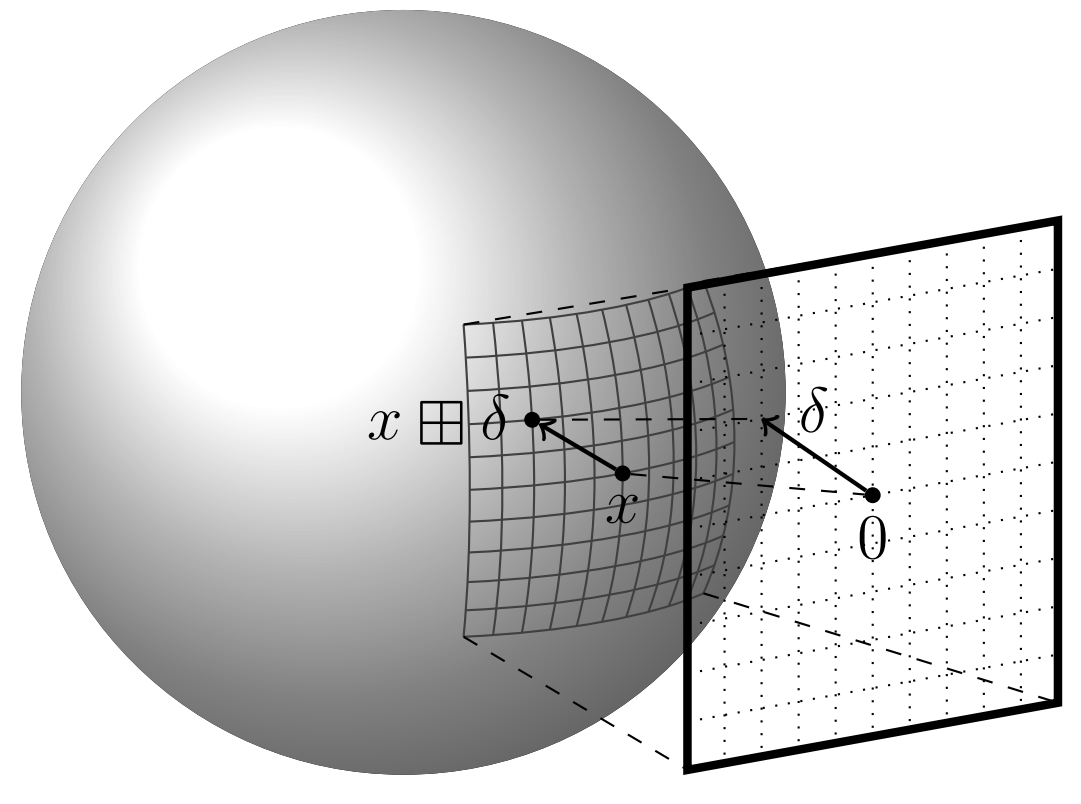
\includegraphics[width=0.7\linewidth]{Pictures/State_Estimation/Unscented_Kalman_Filter_on_Manifolds/Manifold_Mapping.png}
    \caption{Mapping a local neighborhood in the state space (here: on the unit sphere $\mathbb{S}^2$) into $\mathbb{R}^n$ (here: the plane) allows for the use of standard sensor fusion algorithms without explicitly encoding the global topological structure. Image and figure text taken from UKF-M paper.\textsuperscript{\cite{ukf_manifold}}}
    \label{fig:state-estimation-manifold-mapping}
\end{figure}
\noindent
To enable consistent state updates on a nonlinear manifold, the UKF-M introduces two generalized operators, $\boxplus$ and $\boxminus$, which replace standard addition and subtraction. They relate the manifold to its tangent space:
$$
\begin{aligned}
    \mathbf{x}' = \mathbf{x} \boxplus \boldsymbol{\delta} \\
    \boldsymbol{\delta} = \mathbf{y} \boxminus \mathbf{x}
\end{aligned}
$$
Note that $\boldsymbol{\delta}$ is \textit{not} the error state as used in the ESKF formulation. Instead, $\boldsymbol{\delta}$ represents a small perturbation defined in the local tangent space at $\mathbf{x}$, and can take any arbitrary value within that space.  
\\ \\
Here, $\mathbf{x}$ and $\mathbf{y}$ are elements on the manifold $\mathcal{M}$, while $\boldsymbol{\delta} \in T_\mathbf{x}\mathcal{M}$ is the corresponding vector in the tangent space. The $\boxplus$ operator applies a perturbation from the tangent space to move the state along the manifold, producing an updated manifold element $\mathbf{x}'$. Conversely, the $\boxminus$ operator computes the minimal difference between two manifold states by mapping that displacement back into the tangent space.  
\\ \\
Together, these two operators define a consistent way to move back and forth between the manifold $\mathcal{M}$ and its tangent space $T_\mathbf{x}\mathcal{M}$, enabling the UKF-M to perform all statistical operations (eks, mean and covariance propagation) in a locally Euclidean space while keeping the final state representation on the true manifold. 
\\ \\
In Euclidean space, these operators reduce to standard vector addition and subtraction, i.e.
$\mathbf{x}' = \mathbf{x} \boxplus \boldsymbol{\delta} = \mathbf{x} + \boldsymbol{\delta}$ and $\boldsymbol{\delta} = \mathbf{y} \boxminus \mathbf{x} = \mathbf{y} - \mathbf{x}$. However, on curved manifolds like $\mathbb{S}^3$, directly adding vectors can move the state off the manifold, violating its geometric constraints. To address this, the $\boxplus$ and $\boxminus$ operators rely on the exponential and logarithmic maps that move between the manifold and its tangent space:
$$
\begin{aligned}
    \mathbf{x} \boxplus \delta\mathbf{x} = \exp(\delta\mathbf{x}) \circ \mathbf{x} \\
    \mathbf{y} \boxminus \mathbf{x} = \log(\mathbf{y} \circ \mathbf{x}^{-1})
\end{aligned}
$$
where $\circ$ denotes the group composition operator. The exponential map projects a tangent space perturbation onto the manifold, while the logarithmic map computes the smallest displacement between two manifold elements within the tangent space.  
\\ \\
These mappings are directly analogous to the Lie group relations
$$
\begin{aligned}
    R = \exp(\boldsymbol{\omega}^\times) \\
    \boldsymbol{\omega} = \log(R)
\end{aligned}
$$
which connect a rotation matrix $R \in SO(3)$ and its corresponding rotation vector $\boldsymbol{\omega} \in \mathbb{R}^3$. In the UKF-M framework, the same concept generalizes to full state vectors composed of multiple manifold and Euclidean components.  
\\ \\
For attitude estimation using unit quaternions $\mathbf{q} \in \mathbb{S}^3$, these manifold operators take the form
$$
    \mathbf{q}' = \mathbf{q} \boxplus \boldsymbol{\delta} = \mathbf{q} \otimes \exp\!\left(\tfrac{1}{2}\boldsymbol{\delta}\right)
$$
$$
    \boldsymbol{\delta} = \mathbf{q}' \boxminus \mathbf{q} = 2\,\log\!\left(\mathbf{q}^{-1} \otimes \mathbf{q}'\right)
$$
where $\otimes$ denotes quaternion multiplication, and $\exp(\cdot)$ and $\log(\cdot)$ are the quaternion exponential and logarithmic maps on $\mathbb{S}^3$. 
\\ \\
These manifold operators enable the UKF-M to apply local perturbations and corrections within a Euclidean tangent space while ensuring that all updated states remain on the underlying nonlinear manifold. This approach provides numerical stability and geometric consistency, allowing the filter to handle orientation and position states uniformly. Instead of maintaining a separate error state as in the ESKF, the UKF-M implicitly represents uncertainty and corrections through tangent space perturbations managed by the Unscented Transform. As a result, the filter naturally fuses rotational and Euclidean components without requiring Jacobians or repeated re-linearization.































































%%% ===========================================================================================
%%% ===========================================================================================
%%% ===========================================================================================
%%% ===========================================================================================
%%% ===========================================================================================
%%% ===========================================================================================
%%% ===========================================================================================
%%% ===========================================================================================
%%% ===========================================================================================
%%%%% STOPED HERE WILL NEED TO REDO THE ALGORITHM PART CUZ ITS SHOOOTTTTT BUt now at least I knwo how to do that :)
%%% ===========================================================================================
%%% ===========================================================================================
%%% ===========================================================================================
%%% ===========================================================================================
%%% ===========================================================================================
%%% ===========================================================================================
%%% ===========================================================================================
%%% ===========================================================================================
%%% ===========================================================================================



\subsubsection{Filter Algorithm}
The UKF-M algorithm follows the same conceptual stages as other Kalman-type filters but replaces linearization with the Unscented Transform and operates directly on manifolds. The process consists of sigma-point generation, nonlinear propagation, measurement correction, and quaternion normalization.

\textbf{Sigma-point generation:} \\ \noindent
A set of $2L+1$ sigma points is deterministically chosen around the current state estimate:
$$
\begin{aligned}
    \chi_0 &= \mathbf{x} \\
    \chi_i &= \mathbf{x} + (\sqrt{(L + \lambda)P})_i,          && i = 1, \ldots, L \\
    \chi_i &= \mathbf{x} - (\sqrt{(L + \lambda)P})_{i - L},    && i = L+1, \ldots, 2L
\end{aligned}
$$
Each sigma point is weighted using predefined coefficients $w_i^m$ and $w_i^c$ for mean and covariance reconstruction.

\textbf{Prediction:} \\ \noindent
All sigma points are propagated through the nonlinear INS process model $f(\cdot)$ defined in Equations \ref{eq:kinematics-motion-model}–\ref{eq:kinematics-motion-model-states}, and mapped back to the manifold using the $\boxplus$ operator:
$$
    \chi_i^- = f(\chi_i, \mathbf{u}) \quad \text{and} \quad
    \mathbf{x}^- = \sum_i w_i^m \chi_i^-.
$$
The predicted covariance is computed as
$$
    P^- = \sum_i w_i^c [\chi_i^- \boxminus \mathbf{x}^-][\chi_i^- \boxminus \mathbf{x}^-]^\top + Q.
$$

\textbf{Correction:} \\ \noindent
Sigma points are passed through the nonlinear GNSS measurement model $h(\cdot)$ defined in Equation \ref{eq:aiding-measurement-model} to obtain predicted measurements $\mathbf{z}_i = h(\chi_i^-)$.  
The predicted measurement mean and covariance are
$$
\mathbf{z}^- = \sum_i w_i^m \mathbf{z}_i, \qquad
S = \sum_i w_i^c [\mathbf{z}_i - \mathbf{z}^-][\mathbf{z}_i - \mathbf{z}^-]^\top + R.
$$
The cross covariance between the state and measurement is
$$
P_{xz} = \sum_i w_i^c [\chi_i^- \boxminus \mathbf{x}^-][\mathbf{z}_i - \mathbf{z}^-]^\top.
$$
The Kalman gain and posterior estimate are then
$$
K = P_{xz} S^{-1}, \qquad
\mathbf{x}^+ = \mathbf{x}^- \boxplus (K [\mathbf{z} - \mathbf{z}^-]), \qquad
P^+ = P^- - K S K^\top.
$$

\textbf{Quaternion normalization:} \\ \noindent
After each update, quaternion components are renormalized to maintain a unit-norm attitude representation:
$$
    \mathbf{q}^+ \leftarrow \frac{\mathbf{q}^+}{\|\mathbf{q}^+\|}.
$$
This ensures consistent orientation tracking and prevents numerical drift.



\subsubsection{Advantages and Practical Aspects}
The UKF-M provides several advantages over linearization-based filters. It does not require Jacobians, thereby avoiding errors introduced by incorrect linearization and discretization. It also preserves full second-order accuracy for nonlinear mean and covariance propagation, which improves estimation consistency in strongly nonlinear systems. The manifold formulation ensures consistent quaternion handling without relying on small-angle approximations, maintaining proper orientation representation throughout the estimation process. Furthermore, the approach generalizes naturally to mixed Euclidean-manifold state spaces, enabling unified estimation of position, velocity, attitude, and sensor biases within a single framework. 
\\ \\
Alternative sigma-point generation methods, such as spherical simplex sampling, can further improve numerical stability and reduce the number of required samples. After each update, quaternion normalization is applied to preserve unit magnitude and ensure valid attitude representation.




\subsubsection{UKF-M in SLAM and Navigation}
The UKF-M framework is particularly suited for Simultaneous Localization and Mapping (SLAM) and inertial navigation applications. It provides accurate estimation of both position and orientation without the need for Jacobians or linearization, simplifying implementation compared to ESKF while offering similar or better accuracy \cite{ukf_manifold}.  
\\ \\
From a computational perspective, UKF-M trades analytical complexity for additional numerical computation, as it must evaluate the nonlinear dynamics for multiple sigma points. However, in modern embedded and robotic systems, this cost is minor compared to the gains in stability and ease of implementation. For this reason, UKF-M is adopted in this work as the primary state estimation framework for SLAM, balancing geometric consistency, accuracy, and practical simplicity.
